\documentclass[12pt]{article}
\usepackage[margin=1in]{geometry}
\usepackage{amsmath, amsthm, amssymb, amsfonts, pbox, graphicx}
\usepackage[colorlinks = true, linkcolor = black, urlcolor = blue]{hyperref}

\makeatletter
\renewcommand*{\eqref}[1]{%
  \hyperref[{#1}]{\textup{\tagform@{\ref*{#1}}}}%
}
\makeatother

\newtheorem{theorem}{Theorem}
\theoremstyle{definition}
\newtheorem{problem}{Problem}
\renewcommand*{\proofname}{Solution}
\newenvironment{custompbm}[1]
  {\renewcommand\theproblem{#1}\problem}
  {\endproblem}
\renewcommand{\theenumi}{\alph{enumi}}

\newcommand{\E}{\text{E}}
\newcommand{\V}{\text{Var}}
\newcommand{\Co}[2]{\text{Cov}\left({#1}, {#2}\right)}
\newcommand{\pdf}{\text{pdf}}
\newcommand{\pmf}{\text{pmf}}
\newcommand{\me}{\mathrm{e}}
\newcommand*\diff{\mathop{}\!\mathrm{d}}
\newcommand{\vect}[1]{\boldsymbol{#1}}
\newcommand{\mx}[1][t]{\mu_X({#1})}
\newcommand{\gx}[2]{\gamma_X({#1}, {#2})}
\newcommand\norm[1]{\left\lVert#1\right\rVert}

\graphicspath{ {images/} }

\title{MATH 635 Final Assessment}
\author{Matthew Tiger}


\begin{document}


\maketitle


\begin{problem}{1}
  Suppose that the number of claims each policy holder will have in a given year is
  Poisson distributed with mean randomly distributed with density function $g(\lambda) = e^{-\lambda}$
  for $\lambda \geq 0$.
  What is the probability that a policy holder will have $n$ claims in that year?
\end{problem}

\begin{proof}
  Let $X$ be the discrete random variable representing the number of claims
  a policy holder will have in a given year. Let $Y$ be the continuous random
  variable representing the Poisson parameter $\lambda$ with density function
  $g(\lambda) = e^{-\lambda}$ with $\lambda \geq 0$.

  Conditioning the probability that $X = n$ on the random variable $Y$ shows
  that
  \begin{align*}
    P(X = n) &= \int_{-\infty}^{\infty} P(X=n | Y=\lambda) g(\lambda) d \lambda \\
    &= \int_{0}^{\infty} P(X=n | Y=\lambda) e^{-\lambda} d \lambda
  \end{align*}
  where the limits of integration have changed since $P(X=n | Y=\lambda) = 0$ for
  $\lambda < 0$ given our initial assumptions. Using the probability mass function
  for the Poisson random variable $X$ in conjunction with the fact that for
  $Y=\lambda$ the random variable $X$ will have parameter $\lambda$,
  we see that
  \begin{align*}
    P(X=n | Y=\lambda) = \frac{e^{-\lambda}\lambda^n}{n!}.
  \end{align*}
  Thus, from the above computation, we have that
  \begin{align*}
    P(X = n) &= \int_{0}^{\infty}  e^{-\lambda} \left[\frac{e^{-\lambda}\lambda^n}{n!}\right] d \lambda \\
    &= \frac{1}{n!}\int_{0}^{\infty} \lambda^n e^{-2\lambda} d\lambda.
  \end{align*}
  Making the $u$-substitution $u=2\lambda$, the previous integral transforms into
  \begin{align*}
    P(X = n) &= \frac{1}{n!}\int_{0}^{\infty} 2^{-(n+1)}u^{n} e^{-u} du \\
    &= \frac{2^{-(n+1)}}{n!}\int_{0}^{\infty} u^{n} e^{-u} du \\
    &= \frac{2^{-(n+1)}\Gamma(n+1)}{n!} \\
    &= 2^{-(n+1)},
 \end{align*}
 where we have used the fact that, for an integer $k$,
 \begin{align*}
   \Gamma(k) = \int_0^\infty x^{k-1} e^{-x} dx = (k-1)!.
 \end{align*}

 Therefore, the probability a policy holder will have $n$ claims in that year is $2^{-(n+1)}$.
\end{proof}
\newpage


\begin{problem}
  Consider the differential equation
  \begin{align}\label{diffeq}
    y'' - y = -x,\quad  0<x<1 \quad y(0) = y(1) = 0
  \end{align}
  as in Example 15.12 on page 502.
  Use the basis $\{\phi_j(x)\} = \{x^j(1-x)^j\}$, as in section 15.5.1, to
  compute approximations to the exact solution using the finite-element method.

  Provide relative errors at the points 0.25, 0.50, and 0.75 of the approximations
  using the first $n=2,3,4$ basis functions. Plot
  the corresponding approximations $y_2$, $y_3$, $y_4$, and the exact solution
  $y$. Then find the first value of $j$ for which the relative error at all
  three points is less than 0.5\%.
\end{problem}

\begin{proof}
  The differential equation presented in the problem is a second order linear
  differential equation. It is easily shown that the homogeneous solution is
  given by $y_h(x) = c_1 e^{-x} + c_2e^{x}$ and that a particular solution is
  given by $y_p(x) = x$. Thus the general solution is $y(x) = c_1 e^{-x} + c_2e^{x} + x$.
  Using the boundary conditions, we see that the exact solution is
  \begin{align}\label{exact}
    y(x) = \frac{e^{x}e}{1-e^2} -\frac{e^{-x}e}{1-e^2} + x
  \end{align}

  We now wish to approximate the exact solution $y(x)$.
  Note that the exact solution to the differential equation \eqref{diffeq} is
  a continuous function. This fact combined with the fact that $\{\phi_j(x)\}$
  form a basis of the function space shows that the continuous function $y(x)$
  can be approximated with a linear combination of the basis functions.
  Therefore, we wish to find an approximation $y_n(x)$ to the exact solution
  $y(x)$ where
  \begin{align}\label{finite_approximation}
    y_n(x) = \sum_{j=1}^n a_j \phi_j(x).
  \end{align}
  Note that our basis functions $\{\phi_j(x)\}$ satisfy the boundary
  conditions, i.e.\ $\phi_j(0) = \phi_j(1) = 0$ so that $y_n(x)$ also satisfies the
  boundary conditions.

  Corollary 15.2 suggests that if
  \[
    \int_0^1 (y_n'' - y_n + x)\phi_i(x) dx = 0 \quad \text{for $i=1,\dots,n$}
  \]
  then $y_n'' - y_n + x = 0$, i.e\ $y_n(x)$ satisfies the differential
  equation \eqref{diffeq}. If $y_n(x)$ satisfies the
  differential equation and the boundary conditions, then we know that $y_n(x)$
  approximates the exact solution $y(x)$.

  Therefore, we choose the coefficients $a_j$ such that they satisfy the system of
  equations
  \begin{align}\label{first_system}
    \sum_{j=1}^n a_j \int_0^1 \phi_j''(x)\phi_i(x) - \phi_j(x)\phi_i(x) dx = -\int_0^1 x \phi_i(x) dx \quad \text{for $i=1,\dots,n$}.
  \end{align}

  The above system unnecessarily uses the second derivative of the basis
  functions. We can rewrite the coefficients of the above system to use only
  the first derivative of the basis functions. To see this,
  note that we can rewrite the differential equation \eqref{diffeq} in the form
  \begin{align}\label{alternate_diffeq}
    (p(x)y')' + q(x)y' + r(x)y = f(x)
  \end{align}
  by choosing $p(x) = 1$, $q(x) = 0$, $r(x) = -1$, and $f(x) = -x$. With this form of the
  differential equation we would require the approximation \eqref{finite_approximation}
  to satisfy the following equations
  \[
    \int_0^1 ((p(x)y_n')' + r(x)y_n)\phi_i(x) dx = \int_0^1f(x)\phi_i(x)dx \quad \text{for $i=1,\dots,n$}.
  \]
  Making use of the fact that the basis functions are 0 on the boundary we see that
  \begin{align*}
    \int_0^1(p(x)y_n')'\phi_i(x) dx
    &= \phi_i(x)p(x)y_n'\rvert_0^1 - \int_0^1 p(x)y_n'\phi_i'(x) dx \\
    &= - \int_0^1 p(x)y_n'\phi_i'(x) dx.
  \end{align*}
  With this and the definitions of the functions $p(x)$, $r(x)$, and $f(x)$,
  the system of equations \eqref{first_system} becomes
  \begin{align}\label{system_imp}
    \sum_{j=1}^n a_j \int_0^1 -\phi_j'(x)\phi_i'(x) - \phi_j(x)\phi_i(x) dx = -\int_0^1 x \phi_i(x) dx \quad \text{for $i=1,\dots,n$}.
  \end{align}

  Finding the solution to the system of equations \eqref{system_imp} identifies
  the coefficients $a_j$ that define our approximation.

  In this instance, we have chosen the basis $\left.\{\phi_j(x)\}\right._{j=1}^n$ where $\phi_j(x) = x^j(1-x)^j$.
  Thus,
  \begin{align*}
    \phi_j'(x)
    &= \left(x^j\right)'(1-x)^j + x^j\left((1-x)^j\right)' \\
    &= jx^{j-1}(1-x)^j -jx^j(1-x)^{j-1}
  \end{align*}
  for $j=1,\dots,n$.
\end{proof}

\begin{problem}
  Repeat problem 2 with the basis $\{ \sin(j\pi x)\}$.
\end{problem}

\begin{proof}
  We use the same methods outlined in the solution to problem 2 to obtain an
  approximation using the basis $\{\phi_j(x) \}$ with $\phi_j(x) = \sin(j\pi x)$.
  Now we see see that,
  \begin{align*}
    \phi_j'(x)
    &= j\pi \cos(j\pi x)
  \end{align*}
  for $j=1,\dots,n$.

  Using the MATLAB function $\texttt{approximation.m}$, we construct the above
  system of equations and solve them arriving at approximations to the exact
  solution for $n=2,3,4$.
  The tables comparing the exact solution to these approximations at the
  points $x=0.25, 0.50, 0.75$ can be found below.

  \begin{table}[h!]
    \centering
    \bgroup
    \def\arraystretch{1.75}
    \begin{tabular}{| l | c | c | c | c |}
      \hline
      $x$ & $y(x)$ & $y_{2}(x)$ & $|y(x) - y_{2}(x)|$ & \pbox{5cm}{$\frac{100|y(x) - y_{2}(x)|}{|y(x)|}$} \\
      \hline
      0.25 & 3.504760e-02 & 3.355071e-02 & 1.496893e-03 & 4.271028 \\
      0.50 & 5.659056e-02 & 5.856881e-02 & 1.978250e-03 & 3.495724 \\
      0.75 & 5.027579e-02 & 4.927810e-02 & 9.976905e-04 & 1.984435 \\
      \hline
    \end{tabular}
    \egroup
    \caption{Comparison of approximation $y_{2}$ to solution $y$ using basis $\phi_j = \sin(j\pi x)$. All computations are rounded to 6 significant digits.}
  \end{table}

  \begin{table}[h!]
    \centering
    \bgroup
    \def\arraystretch{1.75}
    \begin{tabular}{| l | c | c | c | c |}
      \hline
      $x$ & $y(x)$ & $y_{3}(x)$ & $|y(x) - y_{3}(x)|$ & \pbox{5cm}{$\frac{100|y(x) - y_{3}(x)|}{|y(x)|}$} \\
      \hline
      0.25 & 3.504760e-02 & 3.522118e-02 & 1.735810e-04 & 0.495272 \\
      0.50 & 5.659056e-02 & 5.620640e-02 & 3.841569e-04 & 0.678836 \\
      0.75 & 5.027579e-02 & 5.094857e-02 & 6.727834e-04 & 1.338186 \\
      \hline
    \end{tabular}
    \egroup
    \caption{Comparison of approximation $y_{3}$ to solution $y$ using basis $\phi_j = \sin(j\pi x)$. All computations are rounded to 6 significant digits.}
  \end{table}

  \begin{table}[!h]
    \centering
    \bgroup
    \def\arraystretch{1.75}
    \begin{tabular}{| l | c | c | c | c |}
      \hline
      $x$ & $y(x)$ & $y_{4}(x)$ & $|y(x) - y_{4}(x)|$ & \pbox{5cm}{$\frac{100|y(x) - y_{4}(x)|}{|y(x)|}$} \\
      \hline
      0.25 & 3.504760e-02 & 3.522118e-02 & 1.735810e-04 & 0.495272 \\
      0.50 & 5.659056e-02 & 5.620640e-02 & 3.841569e-04 & 0.678836 \\
      0.75 & 5.027579e-02 & 5.094857e-02 & 6.727834e-04 & 1.338186 \\
      \hline
    \end{tabular}
    \egroup
    \caption{Comparison of approximation $y_{4}$ to solution $y$ using basis $\phi_j = \sin(j\pi x)$. All computations are rounded to 6 significant digits.}
  \end{table}


  We also provide the graphs of these comparisons in Figure \ref{trig_plot}.

  \begin{figure}[h!]
    \begin{center}
      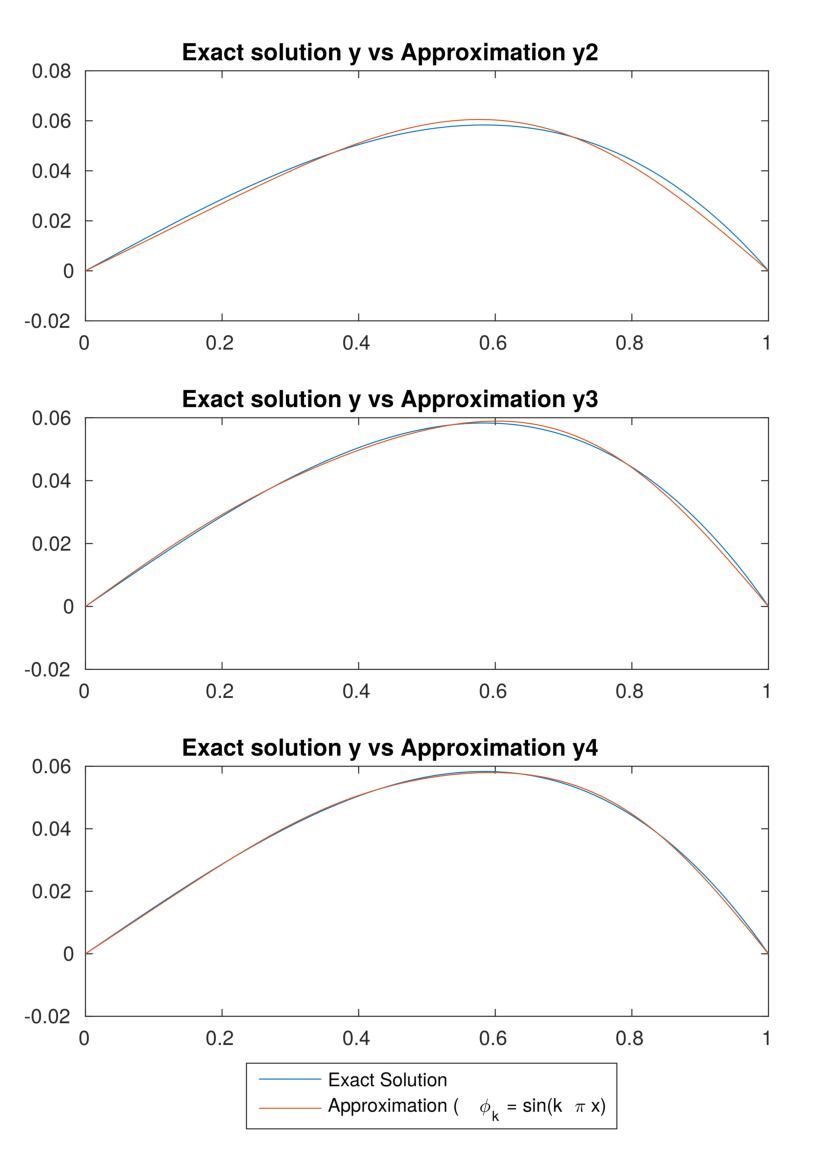
\includegraphics[scale=1.0]{trigonometric_basis_comparison}
    \end{center}
    \caption{Plots of exact solution $y$ and approximation $y_n$ over the interval $[0, 1]$
      using basis $\phi_j = \sin(j\pi x)$.}\label{trig_plot}
  \end{figure}

  The first value of $n$ such that the relative error of the approximation at
  each of the points $x_0=0.25, x_1=0.50, x_2=0.75$ is less than 5.0e-01\% is given by $n=6$.
  The relative errors $r_{x_i}$ at the above points for the approximation $y_6$ are
  $r_{x_0}$ = 3.080284e-01\%, $r_{x_1}$ = 2.293399e-01\%, and $r_{x_2}=$ 2.304205e-02\%.
  This value of $n$ needed for the relative error percents to be less than 5.0e-01\% is quite low.

  The general method of computing the coefficients suits our needs well enough
  if the goal is to obtain an approximation with a relative error less than 5.0e-01\% at these points.
  It will be mentioned, however, that the entries $a_{ij}$ of the coefficient matrix
  found in \eqref{system_imp} admit a special structure due to the choice of basis.
  Namely,
  \begin{align*}
    a_{ij} =
    \begin{cases}
      0 & \text{if $i \neq j$} \\
      \frac{-j^2\pi^2}{2} - \frac{1}{2} & \text{if $i = j$} \\
    \end{cases}
  \end{align*}

  This suggests that the coefficient matrix is actually a diagonal matrix. Finding
  the solution to the system \eqref{system_imp} is therefore trivial and reduces
  the computational complexity of finding the approximation immensely as we only need
  to compute the entries of the coefficient matrix along the diagonal and the entries
  of the column vector in the system. Additionally, a similar calculation shows
  that the integral is not needed for the column vector either as $b_i = (-1)^i / (i\pi)$.

  In order to accommodate this special structure we have created conditional creations
  of the coefficient matrices and column vectors in the code mentioned earlier.
\end{proof}


\begin{problem}
  Repeat the previous problem with the hat function basis (15.51) on p. 502.
\end{problem}

\begin{proof}
  We use the same methods outlined in the solution to problem 2 to obtain an
  approximation using the basis $\{\phi_j(x) \}$. If $n$ is the number of basis functions
  to be used in the approximation, define $h = \frac{1}{n+1}$. Then define the basis function
  as
  \begin{align*}
    \phi_j(x) :=
    \begin{cases}
      \frac{x - h(j-1)}{h} & \text{if $(j-1)h \leq x \leq jh$} \\
      -\frac{x - h(j+1)}{h} & \text{if $jh \leq x \leq (j + 1)h$} \\
      0 & \text{otherwise}. \\
    \end{cases}
  \end{align*}
  Now we see see that,
  \begin{align*}
    \phi_j(x) :=
    \begin{cases}
      \frac{1}{h} & \text{if $(j-1)h < x < jh$} \\
      -\frac{1}{h} & \text{if $jh < x < (j + 1)h$} \\
      0 & \text{otherwise}. \\
    \end{cases}
  \end{align*}
  for $j=1,\dots,n$.

  Note that from our definition of the basis functions that the entry $a_{ij}$
  in the coefficient matrix in the system \eqref{system_imp} is 0 if $|i - j| > 1$.
  This shows that the coefficient matrix is a tri-diagonal matrix and only
  the sub-diagonal, main diagonal, and super-diagonal need to be computed. Additionally,
  as it is clear from the way the entries are defined, the coefficient matrix
  is symmetric and only either the sub-diagonal or super-diagonal needs to be computed.

  Thus, there are only two cases two consider, $i = j$ and $i = j + 1$.
  In the first case, we see that for any $i$,
  \begin{align*}
    a_{ii}
    &= \int_{(i-1)h}^{(i+1)h}-\phi_i'(x)^2 - \phi_i(x)^2 dx \\
    &= \int_{(i-1)h}^{ih} - \left(\frac{1}{h}\right)^2 - \left(\frac{(x - h(i-1))}{h}\right)^2 dx +
    \int_{ih}^{(i+1)h} - \left(-\frac{1}{h}\right)^2 - \left(-\frac{(x - h(i+1))}{h}\right)^2 dx \\
    &= - \frac{2}{h} - \frac{2h}{3}.
  \end{align*}
  In the second case, we similarly see that
  \begin{align*}
    a_{i(i-1)} &=
    \int_{0}^1 -\phi_{i}'(x)\phi_{i-1}'(x) - \phi_{i}(x)\phi_{i-1}(x) dx \\
    &= \int_{(i-1)h}^{ih} -\left(\frac{1}{h}\right)\left(-\frac{1}{h}\right) - \left(\frac{x - h(i-1)}{h}\right)\left(-\frac{(x - hi)}{h}\right)dx
    = \frac{1}{h} - \frac{h}{6}
  \end{align*}
  Therefore,
  \begin{align*}
    a_{ij} =
    \begin{cases}
      - \frac{2}{h} -\frac{2h}{3} & \text{if $i = j$} \\
      \frac{1}{h} - \frac{h}{6} & \text{if $|i - j| = 1$} \\
      0 & \text{otherwise}.
    \end{cases}
  \end{align*}
  The column vector entry is computed very similarly and we see that $b_i = -\frac{i}{(n+1)^2}$.
  These definitions greatly reduce the number of computations needed to compute the coefficient matrix
  and column vector and the integral is no longer needed.

  Using the MATLAB function $\texttt{approximation.m}$, we construct the above
  system of equations and solve them arriving at approximations to the exact
  solution for $n=2,3,4$.

  The tables comparing the exact solution to these approximations at the
  points $x=0.25, 0.50, 0.75$ can be found in Table \ref{hat_1}, Table \ref{hat_2}, and Table \ref{hat_3}.
  As can be seen from the tables, the first $n$ such that the
  relative error percent is less than 0.5\% at each of the points $0.25, 0.50, $ and 0.75
  is $n=3$. Note, however, that for $n=4$ the relative error percent increases at these
  points compared to their values for $n=3$.

  \begin{table}[h!]
    \centering
    \bgroup
    \def\arraystretch{1.75}
    \begin{tabular}{| l | c | c | c | c |}
      \hline
      $x$ & $y(x)$ & $y_{2}(x)$ & $|y(x) - y_{2}(x)|$ & \pbox{5cm}{$\frac{100|y(x) - y_{2}(x)|}{|y(x)|}$} \\
      \hline
      0.25 & 3.504760e-02 &  3.359014e-02 &  1.457462e-03 &  4.158520    \\
      0.50 & 5.659056e-02 &  5.084746e-02 &  5.743100e-03 &  1.014851e01 \\
      0.75 & 5.027579e-02 &  4.268105e-02 &  7.594738e-03 &  1.510616e01 \\
      \hline
    \end{tabular}
    \egroup
    \caption{Comparison of approximation $y_{2}$ to solution $y$ using the hat basis. All computations are rounded to 6 significant digits.}\label{hat_1}
  \end{table}

  \begin{table}[h!]
    \centering
    \bgroup
    \def\arraystretch{1.75}
    \begin{tabular}{| l | c | c | c | c |}
      \hline
      $x$ & $y(x)$ & $y_{3}(x)$ & $|y(x) - y_{3}(x)|$ & \pbox{5cm}{$\frac{100|y(x) - y_{3}(x)|}{|y(x)|}$} \\
      \hline
      0.25 & 3.504760e-02 &  3.521250e-02 &  1.648988e-03 &  4.704996e-01 \\
      0.50 & 5.659056e-02 &  5.685947e-02 &  2.689137e-03 &  4.751917e-01 \\
      0.75 & 5.027579e-02 &  5.051862e-02 &  2.428358e-03 &  4.830075e-01 \\
      \hline
    \end{tabular}
    \egroup
    \caption{Comparison of approximation $y_{3}$ to solution $y$ using the hat basis. All computations are rounded to 6 significant digits.}\label{hat_2}
  \end{table}

  \begin{table}[!h]
    \centering
    \bgroup
    \def\arraystretch{1.75}
    \begin{tabular}{| l | c | c | c | c |}
      \hline
      $x$ & $y(x)$ & $y_{4}(x)$ & $|y(x) - y_{4}(x)|$ & \pbox{5cm}{$\frac{100|y(x) - y_{4}(x)|}{|y(x)|}$} \\
      \hline
      0.25 & 3.504760e-02 &   3.423311 &   8.144879e-04 &  2.323948 \\
      0.50 & 5.659056e-02 &   5.453670 &   2.053859e-03 &  3.629332 \\
      0.75 & 5.027579e-02 &   4.793311 &   2.342679e-03 &  4.659657 \\
      \hline
    \end{tabular}
    \egroup
    \caption{Comparison of approximation $y_{4}$ to solution $y$ using the hat basis. All computations are rounded to 6 significant digits.}\label{hat_3}
  \end{table}

  We also provide the graphs of these comparisons in Figure \ref{hat_plot}.

  \begin{figure}[h!]
    \begin{center}
      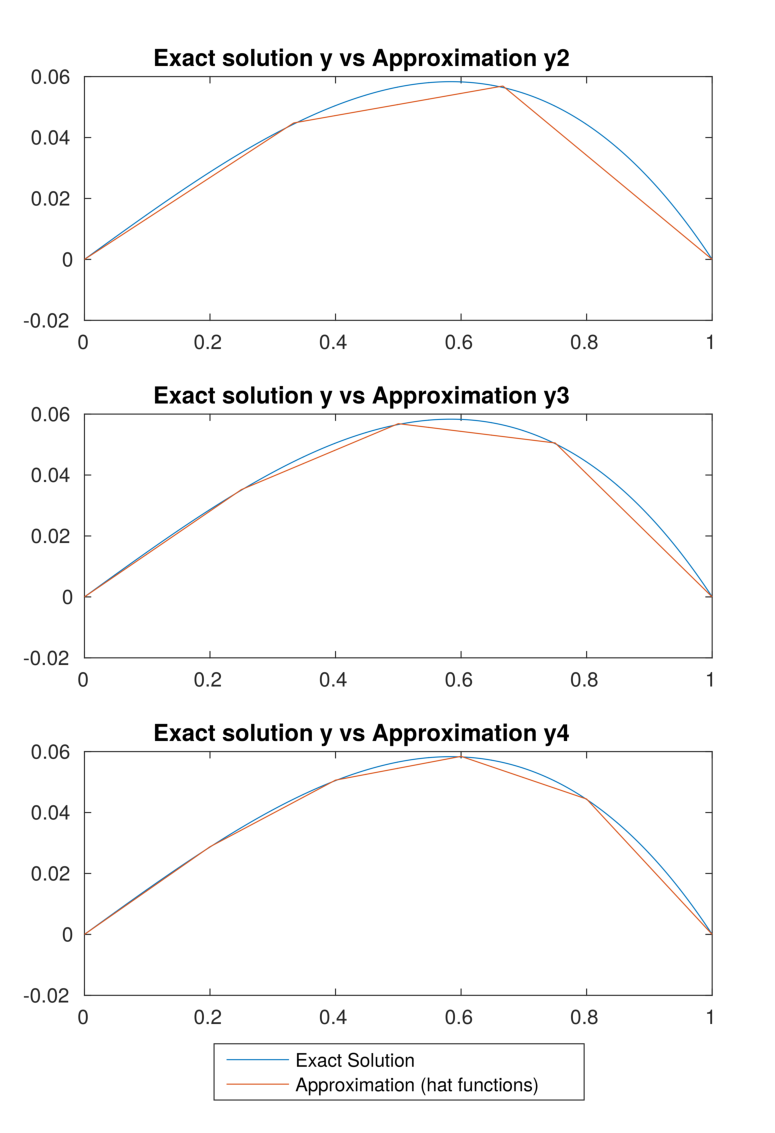
\includegraphics[scale=1.0]{hat_basis_comparison}
    \end{center}
    \caption{Plots of exact solution $y$ and approximation $y_n$ over the interval $[0, 1]$
      using the hat basis.}\label{hat_plot}
  \end{figure}

  The tri-diagonal nature of the coefficient matrix shows that the matrix is sparse.
  MATLAB provides optimized functions for solving systems involving sparse matrices.
  Even though this is not as quick as finding the inverse of a diagonal matrix,
  it is still quite quick in MATLAB. This, coupled with the fact that only at most
  two of the evaluations of the basis functions are needed to compute a point
  on the approximation, shows that this may indeed be the best method for approximating
  the exact solution to this particular differential equation. As such, we have implemented
  special cases of the algorithm for the creation of the coefficient matrix and column vector
  as in the trigonometric basis case.

\end{proof}

\begin{problem}
  Compare the results in problems 2,3,4 and make your recommendation on
  which method is best.
\end{problem}

\begin{proof}
  We now summarize our findings in problems 2, 3, and 4. There are three things
  of interest to us when considering which of these approximations is best:
  \begin{enumerate}
    \item If the approximation attains a relative error percent less than 0.5\%
      at the points 0.25, 0.50, and 0.75 as well as throughout the interval [0, 1].
    \item Number of basis functions needed to attain a relative error percent
      less than 0.5\% at each of the points 0.25, 0.50, and 0.75 as well as throughout the interval [0, 1].
    \item Time and computational power needed to attain a relative error
      percent smaller than 0.5\% at the points 0.25, 0.50, and 0.75 as well as throughout the interval [0, 1].
  \end{enumerate}
  We will investigate these properties for each of the three basis functions.

  From problem 2, we see that the polynomial basis does not practically
  approximate the exact solution for any point outside of small neighborhoods of 0.5.
  As such, we cannot recommend this solution
  as it cannot be used throughout the whole interval of definition in any practical way.

  The trigonometric basis provides great approximations with relative error percents less than 0.5\%
  at the points 0.25, 0.50, and 0.75 as well as throughout the interval [0, 1]
  while also requiring only the first 6 basis functions in order to achieve that accuracy.
  It also appears that the convergence is uniform in the interval of definition suggesting
  that this level of accuracy is a global property and the relative error percent will be in close to 0.5\% for places not near the boundary.
  It is also computationally inexpensive to calculate the entries of the column vector and the coefficients of the
  approximation as the coefficient matrix is a diagonal matrix.

  The hat basis only requires 3 basis functions in order to achieve the given relative error percent
  for the three points. However, as these are linear splines, that accuracy is not attained throughout
  the interval of defintion and as such it is a local property of convergence.
  These errors increase on the next iteration and the errors are not uniform in the
  interval, but it is computationally cheap to compute these approximations.
  The reason for this is that the coefficient matrix
  associated to these basis functions is a sparse matrix and by leveraging MATLAB's system of
  equations solver for sparse coefficient matrices we are able to quickly obtain the
  coefficients needed for the approximation. Additionally only two of the basis functions
  are needed to compute a given point of the approximation as all other basis
  functions will be zero for any given point, reducing the number of computations
  needed to evaluate an approximation.

  In order to obtain more accuracy using the trigonometric basis, you must increase
  the number of basis functions used in the approximation. This has almost no effect on
  solving the system of equations, as there is nothing to solve with a diagonal matrix,
  but computing the values at each of the trigonometric basis functions increases the computational
  cost of using this approximation as you must involve an increasing number of sine functions.
  In contrast, the hat basis allows us to quickly obtain more and more accurate approximations
  requiring more basis functions, but not more computational complexity as only
  two of those functions are needed to provide an approximation for a given point.

  To illustrate this, suppose we are interested in a relative error of 0.0005\%
  at each of the three points 0.25, 0.50, and 0.75. With the trigonometric basis,
  it only took the first 57 basis functions to attain the desired accuracy
  but it took 22.012 seconds to check those basis functions and compute the approximations.
  In contrast, the hat basis functions required the first 123 basis functions,
  but only took 15.581 seconds to check all other basis functions for this degree of accuracy.
  Once the number of basis functions needed for the desired accuracy is determined,
  it is faster to use the basis functions. It only took 2.233 seconds to obtain the
  approximation and compute a point using the basis function compared to the
  3.633 seconds required to obtain the approximation and compute a point. This
  suggests that using the hat basis will be faster if interested in obtaining
  an approximation obtaining a relative error less than 0.5\%.

  In summary, if you are interested in only obtaining a maximum relative error of 0.5\%
  at the given points, you should use the hat basis functions. If you are interested in
  only obtaining a maximum relative error of 0.5\% throughout the interval, you should
  use the trigonometric basis. To obtain more accurate approximations using the least
  amount of time and computational power, it is suggested to use the
  hat basis as it is very cheap computationally to solve the system of equations
  associated to the problem and to evaluate the approximation for higher numbers
  of included basis functions.
\end{proof}

\begin{problem}
  Throughout these last two sections, we have tacitly assumed there exists a unique
  solution. That is not always the case. Consider the problem
  \[
    y'' + y = 0 \quad y(0) = y(\pi) = 0.
  \]

  There are infinitely many solutions, all of the form: $y = C\sin(x)$, where $C$
  is an arbitrary constant. Nevertheless, use the finite-element method to solve
  this problem. Take larger and larger values of $n$. Recall the theory of
  eigenvalues for matrices
\end{problem}

\begin{proof}
  We wish to find an approximation $y_n(x)$ to the exact solution $y = C\sin(x)$
  using the finite-element method employing the hat basis outlined in problem 4.
  The approximation will have the form
  \begin{align*}
    y_n(x) = \sum_{j=1}^n a_j \phi_j(x).
  \end{align*}
  where
  \begin{align*}
    \phi_j(x) :=
    \begin{cases}
      \frac{x - h(j-1)}{h} & \text{if $(j-1)h \leq x \leq jh$} \\
      -\frac{x - h(j+1)}{h} & \text{if $jh \leq x \leq (j + 1)h$} \\
      0 & \text{otherwise} \\
    \end{cases}
  \end{align*}
  and $h = \pi / (n + 1)$.

  Following the methods outlined in problem 2, we want the approximation to
  satisfy the equations
  \begin{align*}
    \int_0^\pi (y_n'' + y_n)\phi_i(x)dx = 0 \quad \text{for $i = 1,\dots,n$}.
  \end{align*}

  In order to practically solve the system, we rewrite the differential
  equation in the form presented in \eqref{alternate_diffeq} by
  choosing $p(x) = 1$, $r(x) = f(x) = 0$, and $q(x) = 1$. Thus,
  the system becomes
  \[
    \int_0^\pi ((p(x)y_n')' + r(x)y_n)\phi_i(x) dx = 0 \quad \text{for $i=1,\dots,n$}.
  \]
  Making use of the fact that the basis functions are 0 on the boundary we see that
  \begin{align*}
    \int_0^\pi (p(x)y_n')'\phi_i(x) dx
    &= \phi_i(x)p(x)y_n'\rvert_0^\pi - \int_0^\pi p(x)y_n'\phi_i'(x) dx \\
    &= - \int_0^\pi p(x)y_n'\phi_i'(x) dx.
  \end{align*}
  With this and the definitions of the functions $p(x)$ and $r(x)$,
  the system of equations becomes
  \begin{align}\label{system_imp}
    \sum_{j=1}^n a_j \int_0^\pi -\phi_j'(x)\phi_i'(x) + \phi_j(x)\phi_i(x) dx = 0\quad \text{for $i=1,\dots,n$}.
  \end{align}

  Proceeding as we did in problem 4, we see that each of the entries $a_{ij}$
  of the coefficient matrix $A$
  has a special structure and that we need only calculate the diagonal and sub-diagonal.

  Thus, there are only two cases two consider, $i = j$ and $i = j + 1$.
  In the first case, we see that for any $i$,
  \begin{align*}
    a_{ii}
    &= \int_{(i-1)h}^{(i+1)h}-\phi_i'(x)^2 + \phi_i(x)^2 dx \\
    &= \int_{(i-1)h}^{ih} - \left(\frac{1}{h}\right)^2 + \left(\frac{(x - h(i-1))}{h}\right)^2 dx +
    \int_{ih}^{(i+1)h} - \left(-\frac{1}{h}\right)^2 + \left(-\frac{(x - h(i+1))}{h}\right)^2 dx \\
    &= - \frac{2}{h} + \frac{2h}{3}.
  \end{align*}
  In the second case, we similarly see that
  \begin{align*}
    a_{i(i-1)} &=
    \int_{0}^1 -\phi_{i}'(x)\phi_{i-1}'(x) + \phi_{i}(x)\phi_{i-1}(x) dx \\
    &= \int_{(i-1)h}^{ih} -\left(\frac{1}{h}\right)\left(-\frac{1}{h}\right) + \left(\frac{x - h(i-1)}{h}\right)\left(-\frac{(x - hi)}{h}\right)dx
    = \frac{1}{h} + \frac{h}{6}
  \end{align*}
  Therefore,
  \begin{align*}
    a_{ij} =
    \begin{cases}
      - \frac{2}{h} + \frac{2h}{3} & \text{if $i = j$} \\
      \frac{1}{h} + \frac{h}{6} & \text{if $|i - j| = 1$} \\
      0 & \text{otherwise}.
    \end{cases}
  \end{align*}
  Thus, our system is given by
  \begin{align*}
    \renewcommand\arraystretch{1.5}
    \begin{bmatrix}
      - \frac{2}{h} + \frac{2h}{3} & \frac{1}{h} + \frac{h}{6} & \hdots & 0 \\
      \frac{1}{h} + \frac{h}{6} & - \frac{2}{h} + \frac{2h}{3} & \hdots & 0 \\
      \vdots & \vdots & \ddots & \vdots  \\
      0 & 0 & \hdots & - \frac{2}{h} + \frac{2h}{3} \\
    \end{bmatrix}
    \begin{bmatrix}
      a_1 \\
      a_2 \\
      \vdots \\
      a_n
    \end{bmatrix}
    =
    \begin{bmatrix}
      0 \\
      0 \\
      \vdots \\
      0 \\
    \end{bmatrix}.
  \end{align*}
  The astute observer will note that the solution to this system is in fact the
  trivial solution. We therefore make the following transformation to the system
  \begin{align*}
    \renewcommand\arraystretch{1.5}
    \begin{bmatrix}
      \frac{2}{h} & -\frac{1}{h} & \hdots & 0 \\
      -\frac{1}{h} & \frac{2}{h} & \hdots & 0 \\
      \vdots & \vdots & \ddots & \vdots  \\
      0 & 0 & \hdots & \frac{2}{h} \\
    \end{bmatrix}
    \begin{bmatrix}
      a_1 \\
      a_2 \\
      \vdots \\
      a_n
    \end{bmatrix}
    &=
    \renewcommand\arraystretch{1.5}
    \begin{bmatrix}
      \frac{2h}{3} & \frac{h}{6} & \hdots & 0 \\
      \frac{h}{6} & \frac{2h}{3} & \hdots & 0 \\
      \vdots & \vdots & \ddots & \vdots  \\
      0 & 0 & \hdots & \frac{2h}{3} \\
    \end{bmatrix}
    \begin{bmatrix}
      a_1 \\
      a_2 \\
      \vdots \\
      a_n
    \end{bmatrix} \\
    A_1 x &= M x \\
  \end{align*}

  The problem then becomes finding the eigenvector solution to the generalized
  eigenvalue problem $A_1 x = \lambda M x$ associated to the eigenvalue $\lambda = 1$.
  Thus, the eigenvector $x$ satisfying the equation is the vector of coefficients
  to use in our approximation.
  Using the MATLAB program \texttt{eigenvector\_approximation.m} we obtain
  an approximation using $n$ nodes to the exact solution.
  The programming code mentioned can be found at the following link:

\url{https://github.com/gammadistribution/gradschool/tree/master/MATH635/final/programs/eigenvector_approximation}

  \begin{figure}[h!]
    \begin{center}
      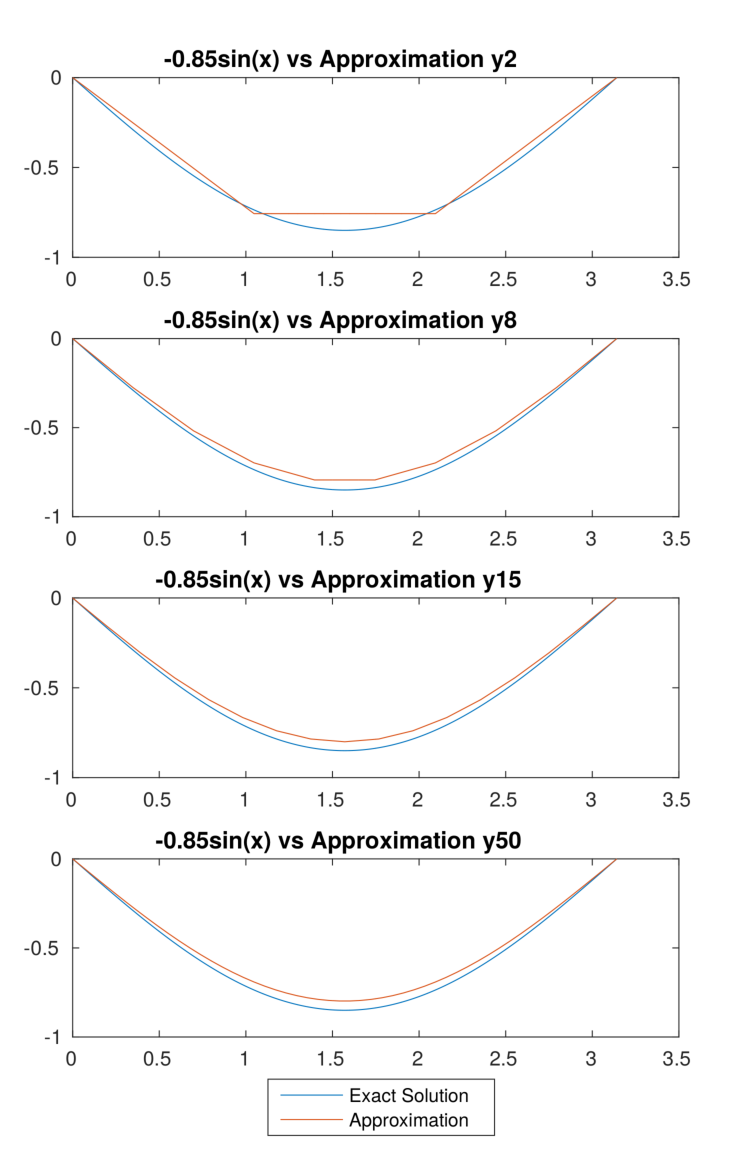
\includegraphics[scale=1.0]{eigenvector_approximation}
    \end{center}
    \caption{Plots of $y=-0.85\sin(x)$ and approximation $y_n$ over the interval $[0, \pi]$
      using the hat basis.}\label{eigen}
  \end{figure}

  We plot the approximations for $n=2, 8, 15, 50$ on the interval $[0, \pi]$
  along with the function $y(x) = -0.85\sin(x)$ in Figure \ref{eigen}. From these
  plots we can see that as we refine the mesh on the interval our approximation
  seems to approach the function $y(x) = C\sin(x)$ for $C = -0.8$ on the interval $[0, \pi]$.
  The function $y(x)=-0.85\sin(x)$ is used as a reference point for the approximation.

\end{proof}



\end{document}
